% Options for packages loaded elsewhere
\PassOptionsToPackage{unicode}{hyperref}
\PassOptionsToPackage{hyphens}{url}
%
\documentclass[
]{article}
\usepackage{lmodern}
\usepackage{amssymb,amsmath}
\usepackage{ifxetex,ifluatex}
\ifnum 0\ifxetex 1\fi\ifluatex 1\fi=0 % if pdftex
  \usepackage[T1]{fontenc}
  \usepackage[utf8]{inputenc}
  \usepackage{textcomp} % provide euro and other symbols
\else % if luatex or xetex
  \usepackage{unicode-math}
  \defaultfontfeatures{Scale=MatchLowercase}
  \defaultfontfeatures[\rmfamily]{Ligatures=TeX,Scale=1}
\fi
% Use upquote if available, for straight quotes in verbatim environments
\IfFileExists{upquote.sty}{\usepackage{upquote}}{}
\IfFileExists{microtype.sty}{% use microtype if available
  \usepackage[]{microtype}
  \UseMicrotypeSet[protrusion]{basicmath} % disable protrusion for tt fonts
}{}
\makeatletter
\@ifundefined{KOMAClassName}{% if non-KOMA class
  \IfFileExists{parskip.sty}{%
    \usepackage{parskip}
  }{% else
    \setlength{\parindent}{0pt}
    \setlength{\parskip}{6pt plus 2pt minus 1pt}}
}{% if KOMA class
  \KOMAoptions{parskip=half}}
\makeatother
\usepackage{xcolor}
\IfFileExists{xurl.sty}{\usepackage{xurl}}{} % add URL line breaks if available
\IfFileExists{bookmark.sty}{\usepackage{bookmark}}{\usepackage{hyperref}}
\hypersetup{
  pdftitle={Package JKGWAS User Tutorial},
  pdfauthor={Pabitra Joshi and Lindsey Kornowske},
  hidelinks,
  pdfcreator={LaTeX via pandoc}}
\urlstyle{same} % disable monospaced font for URLs
\usepackage[margin=1in]{geometry}
\usepackage{color}
\usepackage{fancyvrb}
\newcommand{\VerbBar}{|}
\newcommand{\VERB}{\Verb[commandchars=\\\{\}]}
\DefineVerbatimEnvironment{Highlighting}{Verbatim}{commandchars=\\\{\}}
% Add ',fontsize=\small' for more characters per line
\usepackage{framed}
\definecolor{shadecolor}{RGB}{248,248,248}
\newenvironment{Shaded}{\begin{snugshade}}{\end{snugshade}}
\newcommand{\AlertTok}[1]{\textcolor[rgb]{0.94,0.16,0.16}{#1}}
\newcommand{\AnnotationTok}[1]{\textcolor[rgb]{0.56,0.35,0.01}{\textbf{\textit{#1}}}}
\newcommand{\AttributeTok}[1]{\textcolor[rgb]{0.77,0.63,0.00}{#1}}
\newcommand{\BaseNTok}[1]{\textcolor[rgb]{0.00,0.00,0.81}{#1}}
\newcommand{\BuiltInTok}[1]{#1}
\newcommand{\CharTok}[1]{\textcolor[rgb]{0.31,0.60,0.02}{#1}}
\newcommand{\CommentTok}[1]{\textcolor[rgb]{0.56,0.35,0.01}{\textit{#1}}}
\newcommand{\CommentVarTok}[1]{\textcolor[rgb]{0.56,0.35,0.01}{\textbf{\textit{#1}}}}
\newcommand{\ConstantTok}[1]{\textcolor[rgb]{0.00,0.00,0.00}{#1}}
\newcommand{\ControlFlowTok}[1]{\textcolor[rgb]{0.13,0.29,0.53}{\textbf{#1}}}
\newcommand{\DataTypeTok}[1]{\textcolor[rgb]{0.13,0.29,0.53}{#1}}
\newcommand{\DecValTok}[1]{\textcolor[rgb]{0.00,0.00,0.81}{#1}}
\newcommand{\DocumentationTok}[1]{\textcolor[rgb]{0.56,0.35,0.01}{\textbf{\textit{#1}}}}
\newcommand{\ErrorTok}[1]{\textcolor[rgb]{0.64,0.00,0.00}{\textbf{#1}}}
\newcommand{\ExtensionTok}[1]{#1}
\newcommand{\FloatTok}[1]{\textcolor[rgb]{0.00,0.00,0.81}{#1}}
\newcommand{\FunctionTok}[1]{\textcolor[rgb]{0.00,0.00,0.00}{#1}}
\newcommand{\ImportTok}[1]{#1}
\newcommand{\InformationTok}[1]{\textcolor[rgb]{0.56,0.35,0.01}{\textbf{\textit{#1}}}}
\newcommand{\KeywordTok}[1]{\textcolor[rgb]{0.13,0.29,0.53}{\textbf{#1}}}
\newcommand{\NormalTok}[1]{#1}
\newcommand{\OperatorTok}[1]{\textcolor[rgb]{0.81,0.36,0.00}{\textbf{#1}}}
\newcommand{\OtherTok}[1]{\textcolor[rgb]{0.56,0.35,0.01}{#1}}
\newcommand{\PreprocessorTok}[1]{\textcolor[rgb]{0.56,0.35,0.01}{\textit{#1}}}
\newcommand{\RegionMarkerTok}[1]{#1}
\newcommand{\SpecialCharTok}[1]{\textcolor[rgb]{0.00,0.00,0.00}{#1}}
\newcommand{\SpecialStringTok}[1]{\textcolor[rgb]{0.31,0.60,0.02}{#1}}
\newcommand{\StringTok}[1]{\textcolor[rgb]{0.31,0.60,0.02}{#1}}
\newcommand{\VariableTok}[1]{\textcolor[rgb]{0.00,0.00,0.00}{#1}}
\newcommand{\VerbatimStringTok}[1]{\textcolor[rgb]{0.31,0.60,0.02}{#1}}
\newcommand{\WarningTok}[1]{\textcolor[rgb]{0.56,0.35,0.01}{\textbf{\textit{#1}}}}
\usepackage{graphicx}
\makeatletter
\def\maxwidth{\ifdim\Gin@nat@width>\linewidth\linewidth\else\Gin@nat@width\fi}
\def\maxheight{\ifdim\Gin@nat@height>\textheight\textheight\else\Gin@nat@height\fi}
\makeatother
% Scale images if necessary, so that they will not overflow the page
% margins by default, and it is still possible to overwrite the defaults
% using explicit options in \includegraphics[width, height, ...]{}
\setkeys{Gin}{width=\maxwidth,height=\maxheight,keepaspectratio}
% Set default figure placement to htbp
\makeatletter
\def\fps@figure{htbp}
\makeatother
\setlength{\emergencystretch}{3em} % prevent overfull lines
\providecommand{\tightlist}{%
  \setlength{\itemsep}{0pt}\setlength{\parskip}{0pt}}
\setcounter{secnumdepth}{-\maxdimen} % remove section numbering

\title{Package JKGWAS User Tutorial}
\author{Pabitra Joshi and Lindsey Kornowske}
\date{21 March 2021}

\begin{document}
\maketitle

{
\setcounter{tocdepth}{6}
\tableofcontents
}
~

~

\begin{center}
\textbf{Joshi Kornowske Genome Wide Association Study (JKGWAS)}\par

\includegraphics[width = 0.3\textwidth]{JKGWAS/JKGWAS_logo.png}
\end{center}

~

~

\hypertarget{introduction}{%
\subsubsection{\texorpdfstring{\textbf{Introduction}}{Introduction}}\label{introduction}}

The JKGWAS package provides tools to conduct Genome Wide Association
Study (GWAS) by generalized linear model (GLM) and to visualize the
results. GWAS by GLM improves the true positive detection rate relative
to GWAS by correlation and the functions provided in this package allow
the user to model known covariates and principal components as fixed
effects in addition to the numeric genomic data in order to improve
phenotype prediction. Where applicable, issues related to modeling
non-invertable matrices are automatically solved by detecting Principal
Components with linear dependence on the covariates. GWAS results are
easily visualized by QQ and Manhattan plot functions.

\hypertarget{description-of-package-functions}{%
\subsubsection{\texorpdfstring{\textbf{Description of package
functions}}{Description of package functions}}\label{description-of-package-functions}}

This package ``JKGWAS'' contains a list of functions that you can find
in the git repository and description of which is also mentioned in
``JKGWAS\_0.1.0.pdf''. All the functions have their description,
arguments and parameters clearly mentioned. When you install the package
from github you can see the function and their description just by
typing ??function\_name in the R-console. This will let you know that
what are the input parameters you need to give to get the output.

\hypertarget{getting-started}{%
\subsubsection{\texorpdfstring{\textbf{Getting
started}}{Getting started}}\label{getting-started}}

The devtools package is required to download the JKGWAS package from
Github. If the user has not installed devtools, they should do so by
running the first line in the chunk below.

\begin{Shaded}
\begin{Highlighting}[]
\CommentTok{\#install.packages("devtools", dependencies = TRUE);}
\KeywordTok{library}\NormalTok{(devtools);}
\end{Highlighting}
\end{Shaded}

Once devtools has been installed, the install\(\_\)github() function can
be used to access the JKGWAS package. The following chunk will do this
automatically.

\begin{Shaded}
\begin{Highlighting}[]
\CommentTok{\#install JKGWAS}
\KeywordTok{install\_github}\NormalTok{(}\StringTok{"lindseymaek/HORT545/JKGWAS"}\NormalTok{);}
\KeywordTok{library}\NormalTok{(JKGWAS);}
\end{Highlighting}
\end{Shaded}

The JKGWAS package accepts genomic, phenotype, and covariate data, and
visualizes these with genomic map data. Sample datasets may be found in
the lindseymaek/HORT545 git repository, one level above the JKGWAS
package. All credit for the curation of these datasets belongs to the
Dr.~Zhiwu Zhang laboratory; for more information on these data, the user
should go to . The data are as follows:

\par

\textbullet CROPS545\_Covariates.txt - Covariate (CV) data, with two
factors

\par

\textbullet CROPS545\_Phenotype.txt - Phenotype data

\par

\textbullet mdp\_SNP\_information.txt - Genomic map data

\par

\textbullet mdp\_numeric.txt - Numeric genotype data, with column-wise
snps

\par

Once downloaded to a local directory, import the data as follows:

\begin{Shaded}
\begin{Highlighting}[]
\CommentTok{\#\# define the variable userDataDirectory as the path to the folder in which the datasets are stored}
\NormalTok{userDataDirectory =}\StringTok{ }\KeywordTok{c}\NormalTok{(}\StringTok{"Users/JKGWASdata/examplepath/"}\NormalTok{)}

\CommentTok{\# covariate data}
\NormalTok{CV =}\StringTok{ }\KeywordTok{read.csv}\NormalTok{(}\DataTypeTok{file =} \StringTok{"userDataDirectory/CROPS545\_Covariates.txt"}\NormalTok{, }\DataTypeTok{header =} \OtherTok{TRUE}\NormalTok{, }\DataTypeTok{sep =} \StringTok{""}\NormalTok{);}

\CommentTok{\# genomic map data}
\NormalTok{SNP =}\StringTok{ }\KeywordTok{read.csv}\NormalTok{(}\DataTypeTok{file =} \StringTok{"userDataDirectory/mdp\_SNP\_information.txt"}\NormalTok{, }\DataTypeTok{header =} \OtherTok{TRUE}\NormalTok{, }\DataTypeTok{sep =} \StringTok{""}\NormalTok{);}

\CommentTok{\# numeric genotype data}
\NormalTok{X =}\StringTok{ }\KeywordTok{read.csv}\NormalTok{(}\DataTypeTok{file =} \StringTok{"userDataDirectory/mdp\_numeric.txt"}\NormalTok{, }\DataTypeTok{header =} \OtherTok{TRUE}\NormalTok{, }\DataTypeTok{sep =}\StringTok{""}\NormalTok{);}

\CommentTok{\# phenotype data}
\NormalTok{y =}\StringTok{ }\KeywordTok{read.csv}\NormalTok{(}\DataTypeTok{file =} \StringTok{"userDataDirectory/CROPS545\_Phenotype.txt"}\NormalTok{, }\DataTypeTok{header =} \OtherTok{TRUE}\NormalTok{, }\DataTypeTok{sep =} \StringTok{""}\NormalTok{);}
\end{Highlighting}
\end{Shaded}

The variable names used here correspond to the names of the arguments in
the JKGWAS functions. This is the data that will be used for the
remainder of this tutorial.

In order to simulate phenotype data with QTNs for a desired heritability
value, we also recommend that you utilize the G2P() function also
provided by the Zhang laboratory. This will be used later on in the
tutorial.

\begin{Shaded}
\begin{Highlighting}[]
\CommentTok{\#source G2P}
\KeywordTok{source}\NormalTok{(}\StringTok{"http://www.zzlab.net/StaGen/2021/R/G2P.R"}\NormalTok{)}
\end{Highlighting}
\end{Shaded}

\hypertarget{required-inputs}{%
\subsubsection{\texorpdfstring{\textbf{Required
Inputs}}{Required Inputs}}\label{required-inputs}}

There are three data components required to run the JKGLM() and JKPCA()
functions in JKGWAS, the SNP/marker data, the phenotype data, and the
genetic map data. The map data should contain columns having chromosome
number and positions of each SNP. The JKGLM function will calculate the
pvalues for each SNP as modeled by the user-inputs, these p-values are
required inputs for, the JKQQ and JKManhattan functions.

\par

\textbullet \textbf{SNP/marker data} - The SNP data must be numeric
coded as ``0'', ``1'' and ``2'' where the 0 stands for homozygous for
parent A, 2 stands for homozygous for parent B and 1 is for heterozygous
SNP calls. Below is an example showing the first 5 rows and columns of
our tutorial SNP data.

\begin{Shaded}
\begin{Highlighting}[]
\NormalTok{X[}\DecValTok{1}\OperatorTok{:}\DecValTok{5}\NormalTok{,}\DecValTok{1}\OperatorTok{:}\DecValTok{5}\NormalTok{] }\CommentTok{\#SNP/marker data}
\end{Highlighting}
\end{Shaded}

\begin{verbatim}
##    taxa PZB00859.1 PZA01271.1 PZA03613.2 PZA03613.1
## 1 33-16          2          0          0          2
## 2 38-11          2          2          0          2
## 3  4226          2          0          0          2
## 4  4722          2          2          0          2
## 5  A188          0          0          0          2
\end{verbatim}

\textbullet \textbf{Phenotype data} - The phenotypic data should be
integers, negative or positive that correspond to each individual.To run
the JKGLM function you should first remove the taxa column of the
phenotypic data. Below is the first 5 column and row of phenotypic data
we used in our tutorial.

\begin{Shaded}
\begin{Highlighting}[]
\NormalTok{y[}\DecValTok{1}\OperatorTok{:}\DecValTok{5}\NormalTok{,}\DecValTok{1}\OperatorTok{:}\DecValTok{2}\NormalTok{]}\CommentTok{\#phenotypic data}
\end{Highlighting}
\end{Shaded}

\begin{verbatim}
##    Taxa        Obs
## 1 33-16 -1.2731037
## 2 38-11  0.5515271
## 3  4226 -0.2549273
## 4  4722 -6.1229643
## 5  A188 -2.5939825
\end{verbatim}

\textbullet \textbf{Genetic Map Data} - The other information needed to
run JKGLM package is genetic map of the SNPs. The heading of this map
data should have marker name,chromosome number and chromosome
position.This piece of information will be needed to make manhattan
plot.Below is the first 5 row of map data.

\begin{Shaded}
\begin{Highlighting}[]
\NormalTok{SNP[}\DecValTok{1}\OperatorTok{:}\DecValTok{5}\NormalTok{,}\DecValTok{1}\OperatorTok{:}\DecValTok{3}\NormalTok{]}\CommentTok{\# map data}
\end{Highlighting}
\end{Shaded}

\begin{verbatim}
##          SNP Chromosome Position
## 1 PZB00859.1          1   157104
## 2 PZA01271.1          1  1947984
## 3 PZA03613.2          1  2914066
## 4 PZA03613.1          1  2914171
## 5 PZA03614.2          1  2915078
\end{verbatim}

\hypertarget{optional-inputs}{%
\subsubsection{\texorpdfstring{\textbf{Optional
Inputs}}{Optional Inputs}}\label{optional-inputs}}

\textbullet \textbf{Covariate data} - Finally we have included covariate
data in the package. The covariates mush be integers much like the
phenotype values. If you do not provide the covariate information then
it can also run without the information by using other inputs. The
covariate data should have information on factors. First r row of the
covariate data id shown below.

\begin{Shaded}
\begin{Highlighting}[]
\NormalTok{CV[}\DecValTok{1}\OperatorTok{:}\DecValTok{5}\NormalTok{,}\DecValTok{1}\OperatorTok{:}\DecValTok{3}\NormalTok{] }\CommentTok{\#Covariate data}
\end{Highlighting}
\end{Shaded}

\begin{verbatim}
##    Taxa  FactorA  FactorB
## 1 33-16 2.531331 5.501464
## 2 38-11 2.633860 4.655691
## 3  4226 1.890695 6.136883
## 4  4722 1.856035 7.841858
## 5  A188 2.552629 5.409450
\end{verbatim}

\textbullet \textbf{Principal Components} - Other imputs include the
Principal Components, which can be generated from JKPCA(), or be
provided by the user. The components must be organized columnwise, with
an equal number of observations as X. The user can also determine the
number of principal components to use, with the default being set to
five. The significance threshold (Cutoff) which can be set to the exact
-log(10) of the p-value you want or the default of 0.05/number of SNPs
(Bonferroni Correction). There are also some options you can use to
suppress the plots automatically generated.

\par

\textbullet \textbf{QTN} - The user can provide a vector of the
positions of the known QTNs, in order to visualize the true positive
detection rate by Manhattan plot with JKManhattan().

\hypertarget{outputs-and-examples}{%
\subsubsection{\texorpdfstring{\textbf{Outputs and
Examples}}{Outputs and Examples}}\label{outputs-and-examples}}

After you use the JKGWAS package,the outputs you get includes
information on principal components, p-values of the SNPs, manhattan
plot, QQplot.We can also include the false positives as the
output.Examples of the output are shown below.

\begin{Shaded}
\begin{Highlighting}[]
\CommentTok{\#\# Get Principal Components with JKPCA()}
\NormalTok{PC =}\StringTok{ }\KeywordTok{JKPCA}\NormalTok{(X, CV, }\DataTypeTok{npc =} \DecValTok{10}\NormalTok{);}
\CommentTok{\#\# Perform GWAS by GLM with JKGLM()}
\NormalTok{Pvals =}\StringTok{ }\KeywordTok{JKGLM}\NormalTok{(}\DataTypeTok{X =}\NormalTok{ X, }\DataTypeTok{y =}\NormalTok{ y, CV, PC);}
\CommentTok{\#\# Visualize GWAS by QQ Plot with JKQQ()}
\KeywordTok{JKQQ}\NormalTok{(Pvals);}
\end{Highlighting}
\end{Shaded}

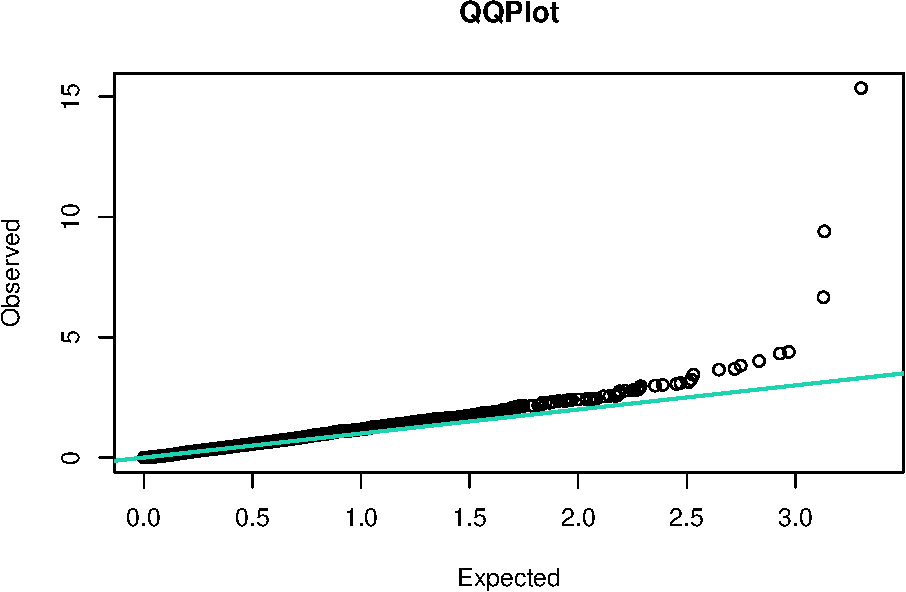
\includegraphics{JKGWAS_UserTutorial_files/figure-latex/unnamed-chunk-10-1.pdf}

\begin{Shaded}
\begin{Highlighting}[]
\CommentTok{\#\# Visualize GWAS by Manhattan Plot with JKManhattan()}
\KeywordTok{JKManhattan}\NormalTok{(}\DataTypeTok{Pvals =}\NormalTok{ Pvals, }\DataTypeTok{SNP =}\NormalTok{ SNP,}\DataTypeTok{sigcutoff =} \OtherTok{NULL}\NormalTok{ );}
\end{Highlighting}
\end{Shaded}

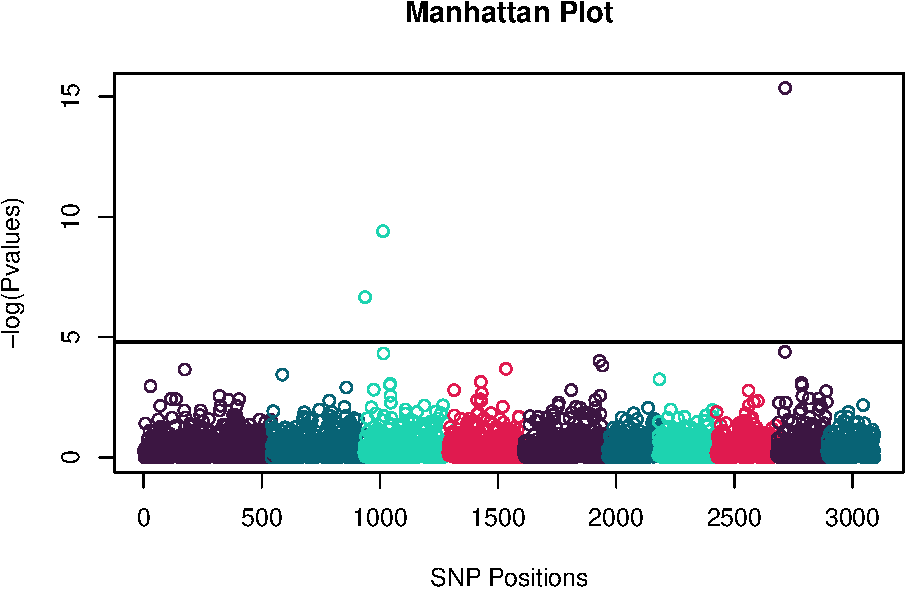
\includegraphics{JKGWAS_UserTutorial_files/figure-latex/unnamed-chunk-10-2.pdf}

\hypertarget{examples-with-known-qtns}{%
\subsubsection{\texorpdfstring{\textbf{Examples with known
QTNs}}{Examples with known QTNs}}\label{examples-with-known-qtns}}

If the user knows the QTNs, they can provide them to the JKManhattan()
function. Alternatively, the G2P() function can be used to simulate
QTNs.

\begin{Shaded}
\begin{Highlighting}[]
\NormalTok{G2P.sim =}\StringTok{ }\KeywordTok{G2P}\NormalTok{(}\DataTypeTok{X=}\NormalTok{ X,}
             \DataTypeTok{h2=} \FloatTok{0.75}\NormalTok{,}
             \DataTypeTok{alpha=}\DecValTok{1}\NormalTok{,}
             \DataTypeTok{NQTN=}\DecValTok{10}\NormalTok{,}
             \DataTypeTok{distribution=}\StringTok{"norm"}\NormalTok{);}

\NormalTok{G2P.y =}\StringTok{ }\KeywordTok{as.data.frame}\NormalTok{(G2P.sim}\OperatorTok{$}\NormalTok{y);}

\NormalTok{Pvals.sim =}\StringTok{ }\KeywordTok{JKGLM}\NormalTok{(}\DataTypeTok{X =}\NormalTok{ X, }\DataTypeTok{y =}\NormalTok{ G2P.y, CV, PC);}

\CommentTok{\#\# Visualize GWAS by QQ Plot with JKQQ()}
\KeywordTok{JKQQ}\NormalTok{(Pvals.sim);}
\end{Highlighting}
\end{Shaded}

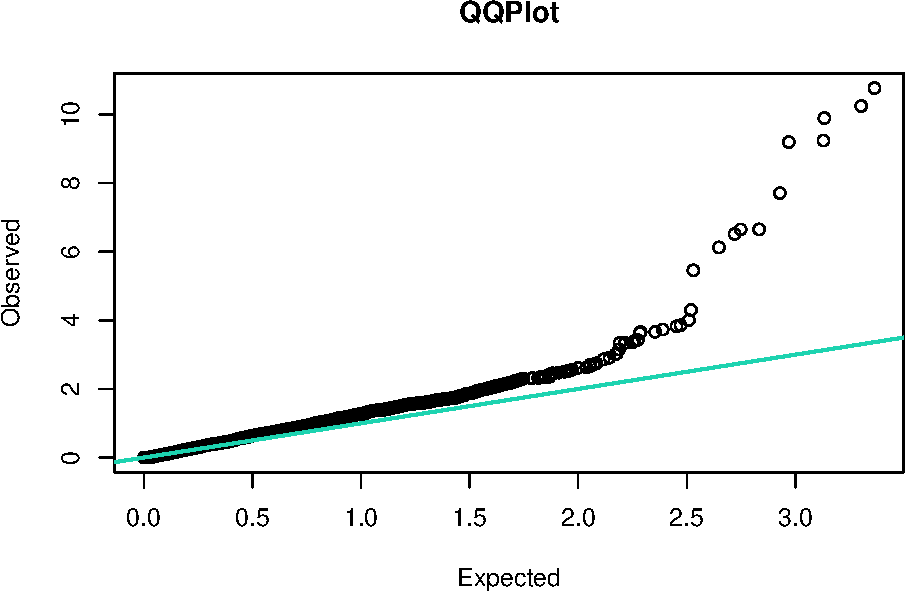
\includegraphics{JKGWAS_UserTutorial_files/figure-latex/unnamed-chunk-11-1.pdf}

\begin{Shaded}
\begin{Highlighting}[]
\CommentTok{\#\# Visualize GWAS by Manhattan Plot with JKManhattan()}
\KeywordTok{JKManhattan}\NormalTok{(}\DataTypeTok{Pvals =}\NormalTok{ Pvals.sim, }\DataTypeTok{SNP =}\NormalTok{ SNP, }\DataTypeTok{sigcutoff =} \OtherTok{NULL}\NormalTok{, }\DataTypeTok{QTN =}\NormalTok{ G2P.sim}\OperatorTok{$}\NormalTok{QTN.position );}
\end{Highlighting}
\end{Shaded}

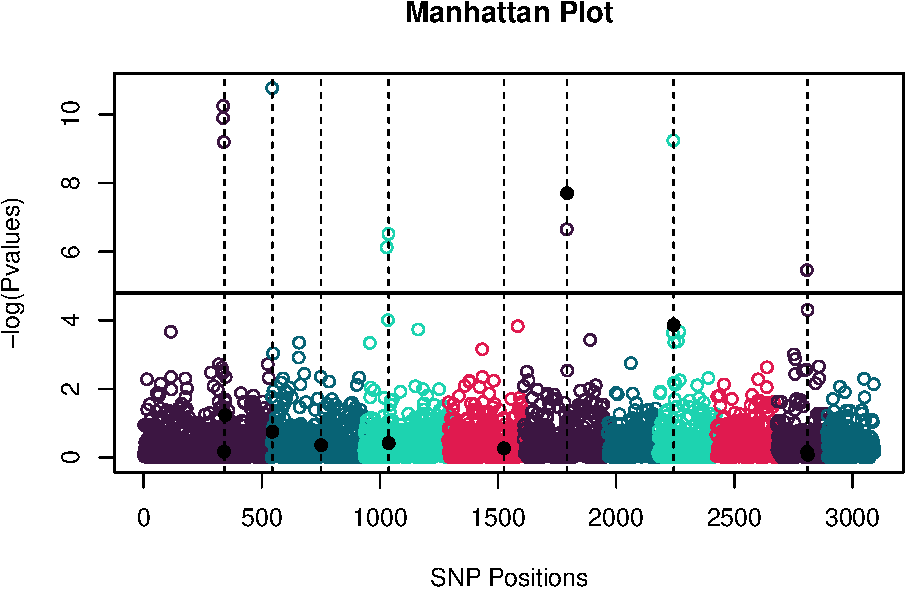
\includegraphics{JKGWAS_UserTutorial_files/figure-latex/unnamed-chunk-11-2.pdf}

\hypertarget{frequently-asked-questions}{%
\subsubsection{\texorpdfstring{\textbf{Frequently asked
questions}}{Frequently asked questions}}\label{frequently-asked-questions}}

\textbf{1. Where can I get JKGWAS?}

\par

JKGWAS is currently available on github via Lindsey Kornowske's public
repository found at \url{https://github.com/lindseymaek/HORT545}

\par

\textbf{2. How do I download JKGWAS?}

\par

Please refer the ``Getting started'' section above where I show how to
download and install JKGWAS using devtools.

\par

\textbf{3. What SNP format does JKGWAS take?}

\par

Currently JKGWAS functions only accept genomic SNP data in the numerical
format. Non-numeric columns will be automatically detected and removed
by the functions.

\par

\textbf{4. What are the required inputs to run JKGWAS?}

\par

You will need SNP data in numerical form, phenotypic data and a genetic
map that has SNP name, Chromosome and position on chromosome. Covariate
data is optional ,but the other three components are prerequisite to run
JKGLM. The output of JKPCA(), can be used as an input for the PC
argument of JKGLM(), and the output of JKGLM() can be used as the input
for the Pvals argument of JKQQ() and JKManhattan().

\textbf{5. Where can I get help with issues regarding JKGWAS}

\par

You can contact the two developer of this package Lindsey Kornowske, at
\href{mailto:lindsey.kornowske@wsu.edu}{\nolinkurl{lindsey.kornowske@wsu.edu}}
and Pabitra Joshi at
\href{mailto:pabitrajoshi77@gmail.com}{\nolinkurl{pabitrajoshi77@gmail.com}}
if you have any questions.

\par

\textbf{6. Are there other R packages that can perform GWAS?}

\par

Yes, the GAPIT package, authored by the Dr.~Zhiwu Zhang laboratory can
be found at \url{http://www.zzlab.net/GAPIT/} and has many advanced
tools for GWAS and visualization.

\par

\hypertarget{further-information}{%
\subsubsection{\texorpdfstring{\textbf{Further
Information}}{Further Information}}\label{further-information}}

More information about GWAS, including sample data, publications, R
packages, and more, can be found at the Zhiwu Zhang Laboratory Website:
\url{http://www.zzlab.net/index.html} If you are a StaGen545 student
from the future - good luck on homework 4, we challenge you to
out-awesome the JKGWAS package logo.

\end{document}
